\section{The mission should leave a better way to work}

A useful project plan answers a present question: which work should start when, with the available crew? A reusable strategy answers a different question: how should the next plan be constructed, checked and repaired? The second object can be productive capital. It also has an acquisition cost, an applicability boundary and a maintenance liability. Keeping every discovered method is therefore an investment policy, not a free improvement.

This edition studies that distinction through the released AGI ALPHA workbench. Its flagship is a finite release-planning service: give it jobs, dependencies, durations, crew needs, a capacity calendar and a deadline; receive a schedule with a separately checked feasibility record. A later requirement can change the calendar and lock already committed work. The system must then repair the plan, account for disruption and decide whether a retained method is still useful. Every example uses disclosed synthetic inputs. A computed schedule is not evidence that the corresponding physical work was performed.

The contribution is an executed, inspectable \emph{strategy-succession experiment}: bounded method search inside the existing workbench, separate correctness and investment gates, fresh mission evaluation, constructive ancestry interventions, recovery records and a browser companion. The strategy grammar contains familiar specialist methods. The scientific claim concerns their construction, selection, reuse and cost in a recurring system; no new general scheduling algorithm or uniquely agentic advantage is assumed.

\begin{insight}[The decisive question]
Can the enterprise discover a better way to work, establish when it helps, retain it, and use it to improve a subsequent worthwhile mission---after paying for the attempt?
\end{insight}

\begin{figure}[ht]\centering
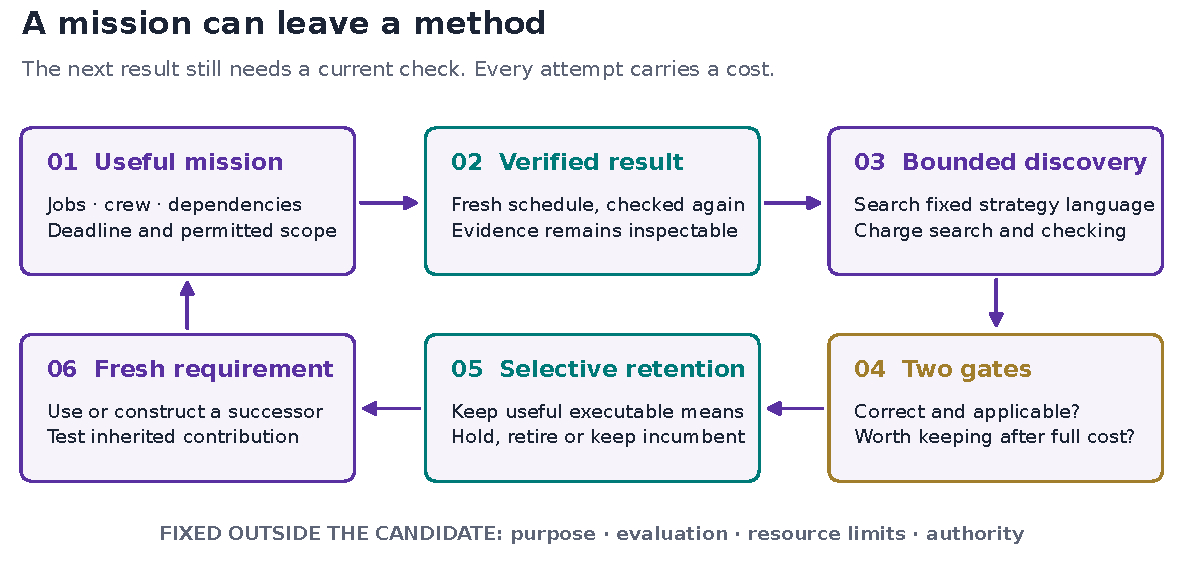
\includegraphics[width=\linewidth]{figures/mission-capability-loop.pdf}
\caption{A productive loop with two gates. Discovery, rejection and upkeep are charged; current purpose, evaluation and authority stay outside candidate control.}\label{fig:loop}
\end{figure}

\subsection{What would count as growth?}

Let $Q_i\in\{0,1\}$ indicate that a fresh mission satisfies its frozen acceptance contract. Let $C_i$ include all declared attributable computational work up to that result, including unsuccessful construction. For cumulative limit $B$, define qualified coverage
\begin{equation}
 K(B)=\sum_i Q_i\,\mathbf{1}\{C_i\leq B\}.
\end{equation}
Coverage is assessed on an offered stream, so an early stop does not remove later missions from the denominator. A rejected or over-budget mission is an observed outcome. Throughput and elapsed time are separately measured; abstract operation charges are never converted silently into seconds or money.

\textbf{Useful reuse} means a retained executable method contributes to a newly checked result. \textbf{Constructive succession} additionally requires that the inherited method helps construct or qualify a semantically different capability. \textbf{Amortized productivity growth} requires a full-cost advantage against a matched strong alternative. \textbf{Capability expansion} requires more qualified fresh missions under the same budget. \textbf{Increasing growth rate} requires improving marginal productivity across matched resource windows, beyond merely repaying an initial cost. \textbf{Commercial growth} requires evidence of demand and economic outcomes. These are separate hypotheses.

The minimum operational claim is narrower: after one explicit start, the finite selector can complete successive permitted phases, preserve history, hold an incumbent, refuse a candidate, wait, recover and stop. Successful execution of that loop does not imply any of the stronger growth claims.

\subsection{Transformational Intelligence as a testable discipline}

The foundational AGI ALPHA paper places governed jobs, verification and reusable capabilities above a particular model \citep{boucher2026agialpha}. Transformational Intelligence separates the mission purpose, its formulation and the means that realize it \citep{boucher2026transformational}. Here the purpose is fixed: produce a valid plan within stated constraints. The system can change the strategy that constructs the plan, while current acceptance criteria remain outside the strategy's control.

This experiment deliberately gives conventional controls the same strategy language. A useful discovered expression therefore establishes strategy learning within that language; it does not establish escape from its attainable set. The possibility of changing a restriction is a research hypothesis that requires a purpose-preserving bridge and its own causal evidence. The symbol $\infty$ expresses the research programme, not an unbounded resource grant or an achieved intelligence level.

\begin{table}[ht]\centering\small
\begin{tabularx}{\linewidth}{L{25mm}YY}
\toprule
Operation & Executed research role & Inspectable output \\
\midrule
Identify & Select the next permitted mission from the frozen queue & Mission, scope, remaining budget and stop/defer decision \\
Out-Learn & Evaluate bounded candidate priorities on disclosed development tasks & Candidate evaluations, failed attempts, acquisition debit \\
Out-Think & Challenge a proposed schedule against original evidence in the separate development probe & Reproducible objection or rejected criticism \\
Out-Design & Construct a typed dispatch, lookahead or repair strategy & Content-bound executable AST and dependency record \\
Out-Strategise & Compare current qualified-output forecasts after full charges & Separate admission decision and break-even conditions \\
Out-Execute & Invoke the unchanged workbench adapter and check its current result & Schedule, check, receipt and cost ledger \\
Out-Evolve & Retain, replace, retire or hold; use permitted means in a later construction & Successor lineage, fresh qualification and removal tests \\
\bottomrule
\end{tabularx}
\caption{Operational counterparts of the six Out-stage papers and Identify. The challenge/adjudication probe is separately executed; it is not an inline model debate in every automatic mission. This mapping does not claim to instantiate every theoretical result in the source papers.}
\end{table}

Out-Learn motivates investing in an experiment; Out-Think motivates checked representations and their retirement; Out-Design emphasizes executable release certificates; Out-Strategise couples information gathering to construction; Out-Execute addresses reusable boundaries and local repair; Out-Evolve makes the durable output a means of further discovery and production \citep{boucher2026outlearn,boucher2026outthink,boucher2026outdesign,boucher2026outstrategise,boucher2026outexecute,boucher2026outevolve}. The present study makes those responsibilities concrete without inheriting their conclusions.
